\documentclass[conference]{IEEEtran}
\IEEEoverridecommandlockouts
% The preceding line is only needed to identify funding in the first footnote. If that is unneeded, please comment it out.
\usepackage{cite}
\usepackage{amsmath,amssymb,amsfonts}
\usepackage{algorithmic}
\usepackage{graphicx}
\usepackage{textcomp}
\usepackage{xcolor}
\def\BibTeX{{\rm B\kern-.05em{\sc i\kern-.025em b}\kern-.08em
    T\kern-.1667em\lower.7ex\hbox{E}\kern-.125emX}}
\begin{document}

\title{Deep Reinforcement Learning for Blackjack}

\author{
    \IEEEauthorblockN{Marius Oechslein}
    \IEEEauthorblockA{
        \textit{Faculty of Computer Science and Business Information Systems} \\
        \textit{University of Applied Sciences Würzburg-Schweinfurt}\\
        Würzburg, Germany \\
        marius.oechslein@study.thws.de
    }
}
\maketitle

% TODO: Main focus of paper:
% . Zuerst implementiere ich "traditional RL-methods" (Sarsa, Q-Learning, TD) als Baseline? 
% . Dann implementiere ich Deep Reinforcement Learning und versuche die Baseline zu erreichen.
% . Dann erhöhe ich den state-space durch das genaue counting aller Karten 
% . -> Hierbei möchte ich vergleichen, wie sich DQN im Vergleich zu traditionellen RL-Methoden verhält. 
% .		Ich habe 3 traditionelle, weil der Test dadurch allgemeingültiger ist und nicht von der Implementierungsdetails einer einzelnen Methode abhängt.


\begin{abstract}
\end{abstract}

\begin{IEEEkeywords}
	Blackjack, Monte Carlo Control, SARSA, Q-Learning, Deep Q-Learning
\end{IEEEkeywords}

\section{Introduction}
\subsection{Blackjack and Reinforcement Learning} 
Blackjack is a popular card game played in casinos worldwide. 
In 1962 the mathematician Edward Thorb published a book containing strategies on how to win at Blackjack \cite{b1}. 
This made it possible for players to win against casinos in the game of Blackjack.
Since then the casinos changed their rules which makes winning for the player impossible now, but the game remains an interesting subject to mathematical modeling due to its probabilistic nature.    

Edward Thorb introduced the idea of card counting with the Complete Point Count System \cite{b1}.
The Complete Point Count System keeps track of a counter that adds +1 or -1 based on each card that are seen by the player. 
This easy counting method makes it possible for players to count cards while playing the game. 

\subsection{Reinforcement Learning for Blackjack}
The game can be modeled as a Markov Decision Process which makes it possible to apply Reinforcement Learning.
The baseline goal is therefore the basic strategy of Edward Thorb \cite{b1} with Reinforcement Learning methods.

All of the Reinforcement Learning methods play a large number of games while keeping track of a Q-Table containing the expected returns to each of the possible game states \cite{b4}.
The different Reinforcement Learning methods like Monte Carlo Control, SARSA and Q-Learning only take a different approach of updating this Q-Table \cite{b4}.
Although they are powerful methods, due to their nature of learning, they require a high amount of games to be able to model the Q-Table as the state-space of the game increases. 
In this paper we hence investigate how well these Reinforcement Learning methods (Monte Carlo Control, SARSA and Q-Learning) perform as we increase the state-space by changing the card counting method. 
We make the card counting method more complex by keeping track of the values of every observed card compared to a single counter in the case of the Complete Point Count System \cite{b1}.

\subsection{Deep Reinforcement Learning}
In 2013 DeepMind combined Deep Learning with Reinforcement Learning in the paper \textit{Playing Atari with Deep Reinforcement Learning} \cite{b2}.
The idea of Deep Reinforcement Learning is to replace the Q-Table with a deep neural network.
This enables estimating Q-Tables for complex state-spaces that traditional Reinforcement Learning methods were unable to.

In this paper we first investigate whether Deep Reinforcement Learning is also able to achieve the baseline of the basic strategy of Edward Thorb \cite{b1}.
Secondly we compare how the Deep Reinforcement Learning method performs compared to the more traditional RL-methods like Monte Carlo Control, SARSA and Q-Learning \cite{b4} as the state-space increases.

% TODO: Do I have the structure of: Establishing niche and occupying niche?


\section{Methods}

\subsection{The Blackjack Environment}
The game of Blackjack starts with the dealer and the player recieving two cards - with the player only seeing one of the dealer's cards and his own hand.
The player then has the two actions to choose from: taking another card (Hitting) and not taking another card (Standing). 
Although the real rules of Blackjack extend this action-space by options like Doubling Down and Splitting, in this paper we only focus on Standing and Hitting. 
It was decided to focus on this reduced action-space since the main points of interest are the Reinforcement Learning methods and not the accurate representation of the game. 

The player can then hit as many times as he wants with the goal of coming as close to a hand value of 21 as possible.
After the player finished his turn the dealer hits as long as his hand value is below or equal 16.
At the end of one game the player's return is two times his bet, his bet or nothing depending on whether it was a win, loss or draw. 
For Reinforcement Learning the rewards is chosen as +1, -1 and 0. 

To model the basic strategy with Reinforcement learning, one game is modeled as one episode. 
It is possible to model only one game as one episode since the basic strategy works only with the information of the dealer's card and the player's hand value while information about the rest of the deck is uninteresting.

When introducing card counting on the other hand, one episode has to be extended to playing multiple games within one episode. 
This is necessary because card counting works with the information of cards already played in addition to the cards of the current game.
The relation between high cards to low cards left in the deck influence the player's chances of winning.
When increasing one episode to playing through a whole deck, the chances of an imbalanced card deck increase which consequently makes card counting more interesting. 

The Complete Point Count System \cite{b1} keeps a running score and updating it every time the player sees a card:
\begin{itemize}
	\item +1 for: 2, 3, 4, 5, 6
	\item -1 for: 10, A
	\item 0 for: 8, 9 
\end{itemize}
It is favourable for the player when the counting score is high \cite{b1}.
And it is favourable for the dealer when the counting score is low.
The main reason for that is that the dealer's chances of busting increases when there are more high cards than low cards left in the deck.

\subsection{State-action space}
For learning the basic strategy the state consists of the \textbf{player's hand value}, the \textbf{dealer's card value} and if the player has an \textbf{usable ace}. 
This makes a total number of \textbf{250 states} that need to be considered:
\begin{itemize}
	\item 10 possible dealer states: 2,3,4,5,6,7,8,9,10,A
	\item 25 possible player states:
		\subitem No Ace: 4,5,6,7,8,9,10,11,12,13,14,15,16,17,18,19,20
		\subitem With Ace: 13,14,15,16,17,18,19,20
\end{itemize}
% player: 2 bis 21 = 2,3,4,5,6,7,9,10,11,12,13,14,15,16,17,18,19,20,21 = 19 

For learning the Complete Point Count System the state has to be extended by a \textbf{counting score}.
The counting score in one episode can at most be +24 (= 6 cards * 4 suits) and at least -20 (= 5 cards * 4 suits).
This would increase the state-space to \textbf{11.000 states} (= 250 states * (24 - 20)) for the Complete Point Count System. 
Although it is important to note that a counting score around 0 is far more likely than of +24 or -20.

When making the card counting method more complex by keeping track of every value of played cards, the state space increases to approximately \textbf{1.048.576.000 states} (= 250 states * (($4^9$ number cards * (4 face cards * 4 states))) for playing through one card deck. 
Unfortunately with such a big state space the calculations ran into RAM problems with the Google Colab Free version (12.7 GB RAM).
For that reason a simpler card counting method was chosen by not keeping track of the exact amount of each of the card-values but only if a card-value has been played or not. 
This can still be informative for predicting the player's chances since it directly tells when all four cards are left in the deck of some card-value.

When using this advanced card counting method the state space is \textbf{1.024.000 states} (= 250 states * (($2^9$ * (4 face cards * 2 states))) when playing through one card deck.

With this huge state space it is interesting to observe how Deep Reinforcement Learning performs and how other Reinforcement Learning methods perform compared to that. 


\subsection{Reinforcement Learning methods}
All of the Reinforcement Learning methods share the basic approach of taking actions in an environment, observing the reward and keeping track of the expected reward to each state-action \cite{b4}.
One more thing that all of the RL-methods have in common is that they have to play a large number of episodes to be able to estimate the expected rewards well \cite{b4}.

Characteristics that the mainly define different RL-methods are the following \cite{b4}:
\begin{itemize}
	\item \textbf{On-policy vs. Off-policy Learning}: If the same policy is used for exploration and exploitation steps. 
	\item \textbf{Update Rule}: With what information the updates are done. 
	\item \textbf{Bootstrapping}: If updates are done based on prediction of future values. 
\end{itemize}

These are the terminologies used for the rest of this paper: 
\begin{itemize}
	\item Q: action-value function
	\item V: state-value function
	\item G: cumulative reward after visited state until the end of the episode 
	\item R: reward
	\item S: state
	\item A: action
	\item t: timestep
	\item $\gamma$: discount rate
	\item $\alpha$: learning rate
\end{itemize}

\subsubsection{Monte Carlo Control}
Monte Carlo Control (MC) was introduced in the book \textit{Reinforcement learning: An introduction} \cite{b4}.
MC is an on-policy learning method which uses the epsilon-greedy method for deciding on whether to take a exploration or an exploitation step.
This is the update rule of Monte Carlo Control:
\begin{equation*}
	V(S_t) \leftarrow V(S_t) + \alpha [G_t - V(S_t)] \tag{1}
\end{equation*}
MC does not use Bootstrapping which means that the updates are calculated based only on real observations. 
This property makes Monte Carlo Control converge slower compared to methods that use Bootstrapping \cite{b4}.  

\subsubsection{SARSA}
The State-Action-Reward-State-Action (SARSA) method was also introduced in the book \textit{Reinforcement learning: An introduction} \cite{b4} and is part of the Temporal Difference Learning methods family.
SARSA is also an on-policy learning method which means that the same policy is used for exploration and exploitation steps which is also done with epsilon-greedy.  
For the update rule, SARSA takes the reward of the next state in consideration:
\begin{equation*}
	Q(S_t, A_t) \leftarrow Q(S_t, A_t) + \alpha [R_{t+1} + \gamma Q(S_{t+1}, A_{t+1}) - Q(S_t, A_t)] \tag{2}
\end{equation*}
This means that SARSA uses bootstrapping since $Q(S_{t+1})$ is used for updating $Q(S_t, A_t)$. 

\subsubsection{Q-Learning}
Q-learning first introduced by Watkins \cite{b5} and taken up in \cite{b4} and also counts as a Temporal Difference Learning method.
Q-learning is an off-policy learning method that uses bootstrapping \cite{b4}:
\begin{equation*}
	Q(S_t, A_t) \leftarrow Q(S_t, A_t) + \alpha [R_{t+1} + \gamma \max_a Q(S_{t+1}, a) - Q(S_t, A_t)] \tag{3}
\end{equation*}


\subsection{Deep Q-Learning}
Deep Q-Learning (DQN) originated in 2013 in the DeepMind paper \textit{Playing Atari with Deep Reinforcement Learning} \cite{b2}.
The main idea of DQN is replacing the Q-Table with a deep neural network \cite{b2}. 
Further, two important implementation details are an \textbf{Experience Replay Buffer} and a \textbf{Target Neural Network} which are presented in the following section.

Pseudo-code for the DQN can be found in the \textit{Playing Atari with Deep Reinforcement Learning} paper \cite{b2}.
For implementation details of the DQN architecture, \textit{Implementing the Deep Q-Network} \cite{b6} is a helpful resource. 
% TODO: For implementation details of the DQN architecture, \textit{Implementing the Deep Q-Network} \cite{b6} and \textit{PyTorch CartPole DQN Tutorial} \cite{} are helpful resources. 

\subsubsection{Experience Replay Buffer} \label{replay-buffer}
At each step of the training loop the Experience Replay Buffer is filled with the Experience of the current training step. 
An Experience consists of:
\begin{itemize}
	\item state
	\item action
	\item reward
	\item next state
\end{itemize}
At every training step a random mini-batch of the Buffer is then sampled and used for the training of the neural network.

The Experience Buffer introduces the advantage of reusing Experiences for training the neural network which increases the data effiency \cite{b2}.
Additionally, sampling random mini-batches uniformly introduces the advantage of breaking the dependency between a state and its preceeding state which helps training a more general neural network \cite{b2}. 

The maximum size of the Buffer is set to 10.000.
When the maximum size is reached, the oldest Experiences are removed and for new Experiences to be added. 

\subsubsection{Target Neural Network}
The traditional Q-Learning method \cite{b4}, the current Q-value is updated by the estimated Q-value of the next state.
To facilitate the same update rule in Deep Q-Learning a target neural network, called $Q^*$ in the DeepMind paper \cite{b2}, is used for predicting the returns of the next state \cite{b6}.
These predicted returns of the next state are then used for the loss function and ultimately for the gradient descent of the learning network \cite{b6}. 

The target network is initialized with the same architecture as the learning neural network.

The weights of the target neural network are fixed and only get updated by the weights of the training network. 
In the paper \cite{b6} this update of the weights is done only every few training steps with the advantage of faster training time. 
In the implementation for this paper, the updates are done every training step but with a update rate of only 0.005 to prevent overfitting.

The advantage of using the target neural network is more stable training and that the errors in estimation are better controlled \cite{b6}.



\section{Experiments and Evaluation}
In the following section the plots of the RL-methods Monte Carlo Control, SARSA and Q-Learning are chosen randomly since these methods perform almost identical. 
The only noticable difference between these RL-methods is their training time.  
The results of the different methods are used interchangably in this section to highlight the simmilarities between these RL-methods and that all of these RL-methods are suitable for the task of modeling Blackjack. 
The second reason why it was decided to not show the plots of all methods is simply because of the number of plots that would need to be shown. 

\subsection{Basic Strategy}
Both the RL-methods and the Deep Q-Learning method come close to the baseline basic strategy of Edward Thorb \cite{b1}.
Figure \ref{fig:monte-carlo-basic-strategy} for example is very close to Edward Thorb's basic strategy for hitting and standing \cite{b1}. 
Although it is important to note that SARSA and Deep Q-Learning  methods needed substantially more training time to achieve this goal than Monte Carlo Control and Q-Learning. 
An exact training time comparison was not conducted since the main focus of this paper is how the methods estimate with increasing state-space and not their training time.

One more important note is that it is unclear what exact rules Edward Thorb used for the calculations in his book \textit{Beat the dealer} \cite{b1}. 
It is therefore unlikely to achieve the exact same basic strategy as Edward Thorb did \cite{b1}.
Although the rules are probably close to the basic Blackjack rules used in the implementation of this paper. 

\begin{figure}
	\centering
	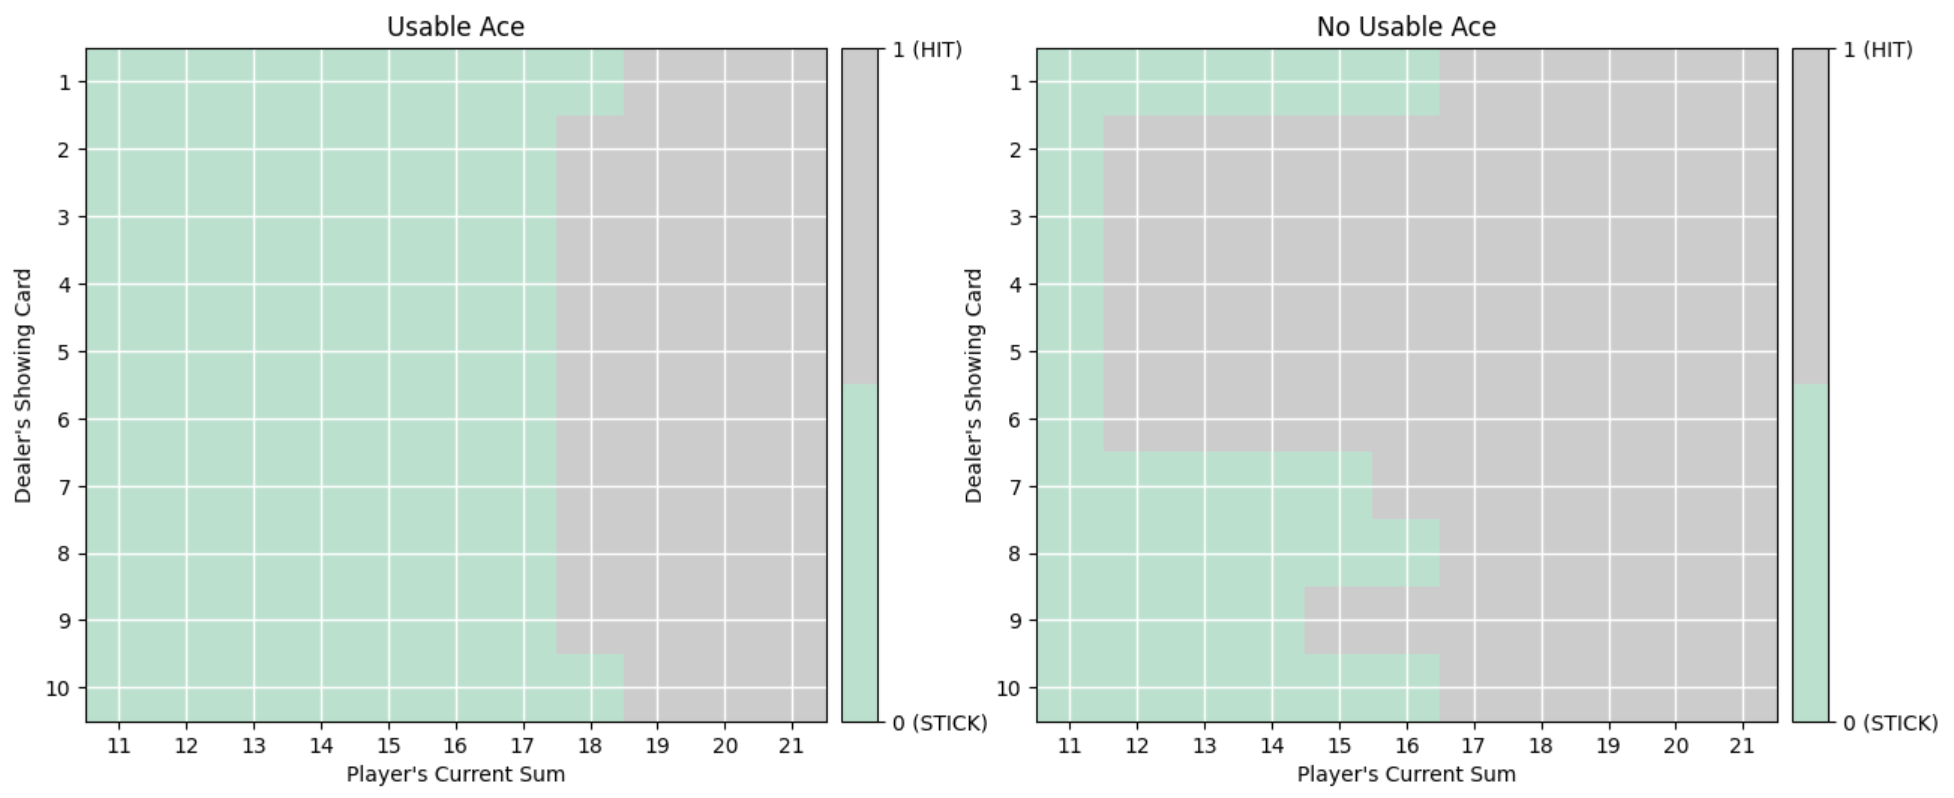
\includegraphics[width=70mm]{figures/MC/basic-100-million/policy.png}
	\caption{Monte Carlo Control policy after 100 million episodes. From own calculations.}
	\label{fig:monte-carlo-basic-strategy}
\end{figure}

In addition to the policy, the state-value function \ref{fig:sarsa-state-value-basic} also looks very close to the state-value function of the basic strategy \cite{b4}.
This indicates that the RL-methods are able to estimate the basic strategy well. 

Note that in Figure \ref{fig:sarsa-state-value-basic} the dealer's ace is shown on the right of its states while in \cite{b4} the ace is shown on the the other side. 

\begin{figure}
	\centering
	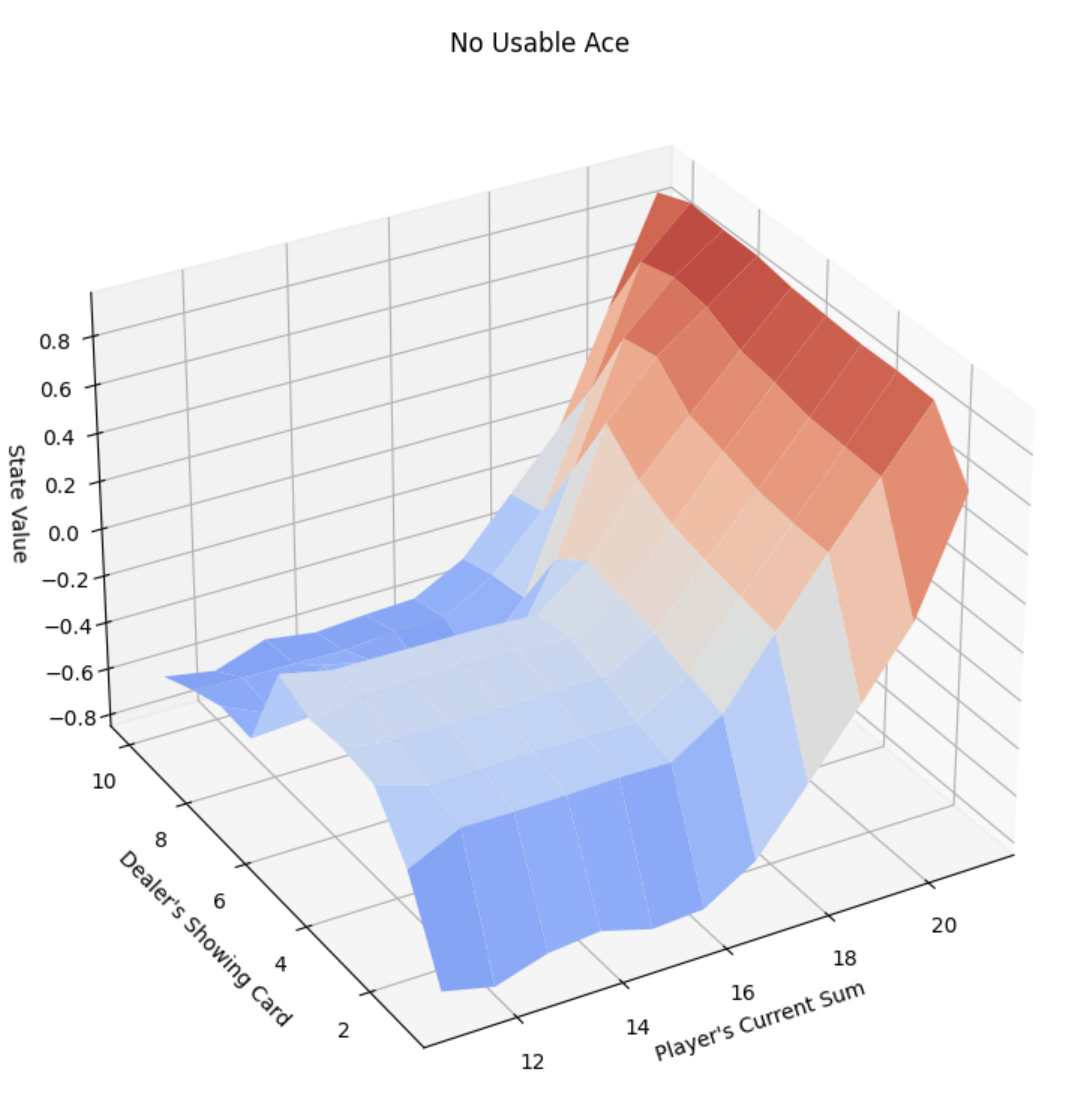
\includegraphics[width=70mm]{figures/MC/basic-100-million/value-function-no-usuable-ace.png}
	\caption{SARSA state-value function after 100 million episodes for case: no-usable ace. From own calculations.}
	\label{fig:sarsa-state-value-basic}
\end{figure}


\subsection{Complete Point Count Sytem}
For the Complete Point Count System the point of interest was whether the player's policy adapts according to the counting score.
A higher counting score indicates that more high cards than low cards are left in the deck as mentioned in the methods section.
This increases the winning chances of the player since there is a higher chance for the dealer to bust \cite{b1}.  

\begin{figure}
	\centering
	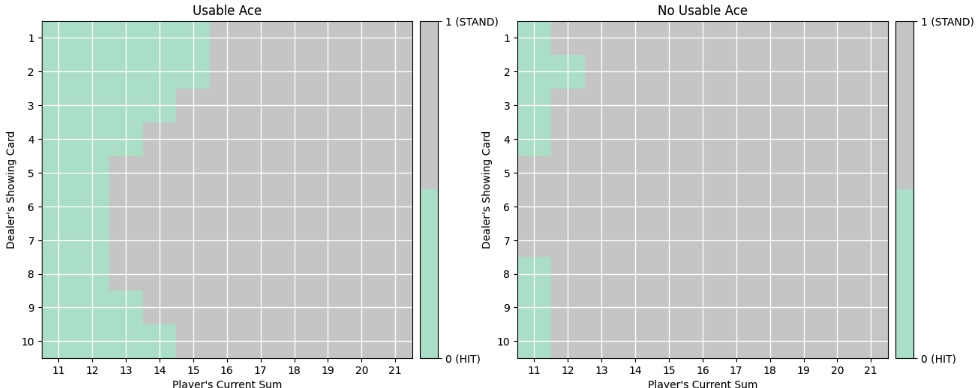
\includegraphics[width=70mm]{figures/DQN/counting-180000/policy-counting-7.png}
	\caption{DQN policy after 180 thousand episodes with a card counting score of 7. From own calculations.}
	\label{fig:dqn-card-counting-7}
\end{figure}

In this state Figure \ref{fig:dqn-card-counting-7} indicates that the player should hit in fewer cases than in the basic strategy in Figure \ref{fig:monte-carlo-basic-strategy}.
This follows Edward Thorb's statement that there is a higher chance for busting which increases the player's winning chances when hitting less \cite{b1}.

Note that for the case where the player has a usable ace, the policy in Figure \ref{fig:dqn-card-counting-5} does not change much. 
This makes sense since the ace's value can be reduced to 1 if the player's hand goes over 21 after hitting a card.
Hitting a card in that case consequently only improves the player's chances of winning which is why he should hit in that case. 


\subsection{Increased state space - counting all cards}
For these experiments a more complex card counting method was used, increasing the state-space to \textbf{1.027.000 states}. 

\subsubsection{Monte Carlo Control, SARSA and Q-Learning}

\begin{figure}
	\centering
	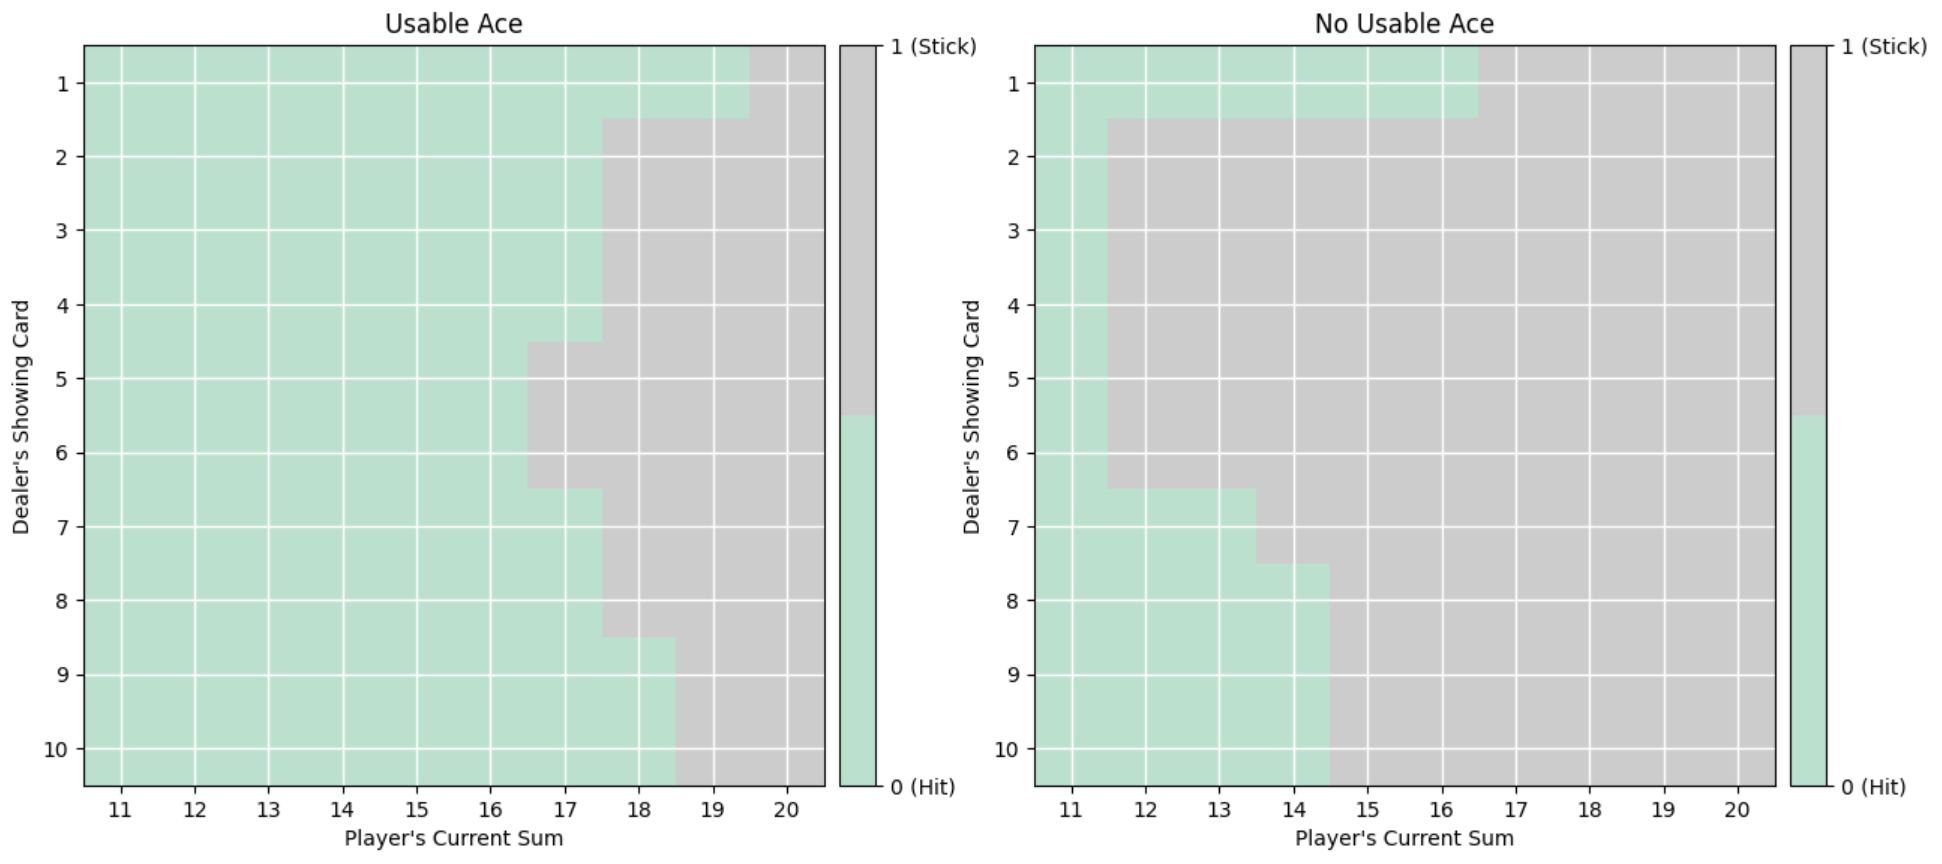
\includegraphics[width=70mm]{figures/Q-Learning/advanced-counting-10-million/policy-all-cards-played-1111111111.png}
	\caption{Q-Learning with advanced counting method. All cards have been played. From own calculations.}
	\label{fig:q-learning-advanced-all-cards-played}
\end{figure}

Figure \ref{fig:q-learning-advanced-all-cards-played} suggest that the policy for the state where are cards have been played at least once is close to the basic strategy from Figure \ref{fig:monte-carlo-basic-strategy}.
It is important to note here that this is the most common state and the policy should thus come close the policy for the basic strategy \cite{b1}.

Notably the policy with this advanced counting method differs a little bit from the basic strategy which is probably due to an insufficient amount of games played in this state.
Even though this state is the most common it is still uncertain to reach this state in every episode.

\begin{figure}
	\centering
	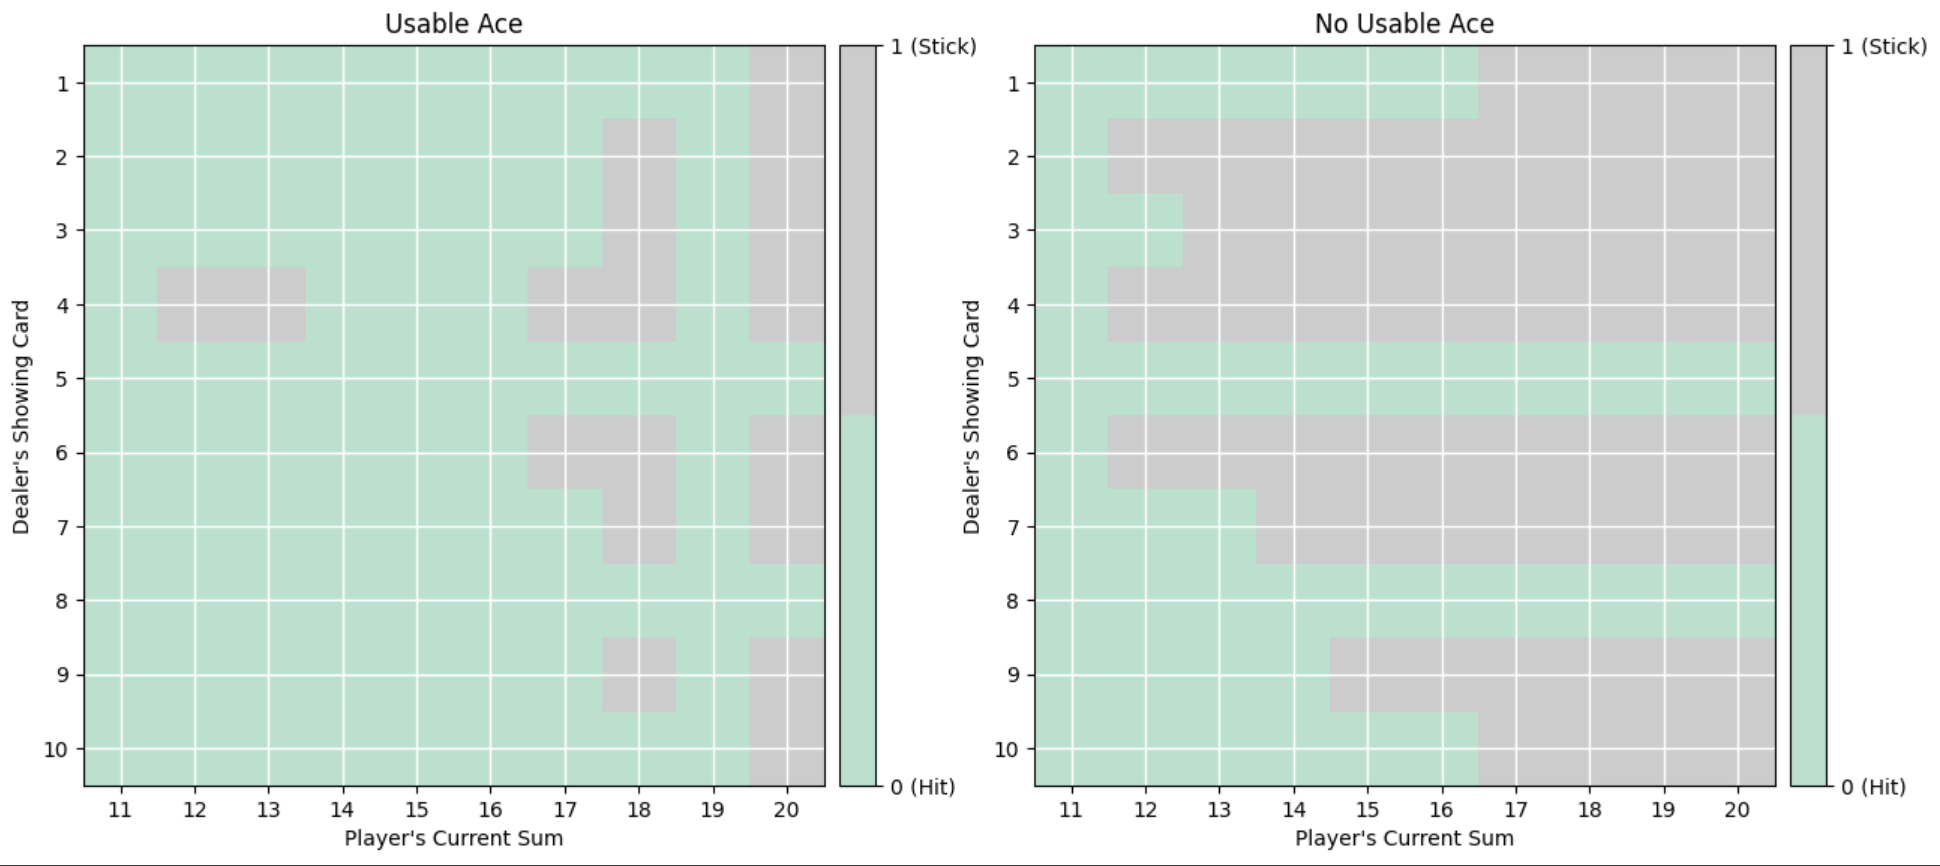
\includegraphics[width=70mm]{figures/Q-Learning/advanced-counting-10-million/policy-5-8-not-played.png}
	\caption{Q-Learning with advanced counting method. Only 5 and 8 have not been played. From own calculations.}
	\label{fig:q-learning-advanced-5-8-not-played}
\end{figure}

In Figure \ref{fig:q-learning-advanced-5-8-not-played} only the cards 5 and 8 have been played. 
This policy is more noisy since this state is less likely than the state from Figure \ref{fig:q-learning-advanced-all-cards-played}.
Hence, there has not been a sufficient amount of games in this state for the RL-method to be able to estimate the policy well.

\begin{figure}
	\centering
	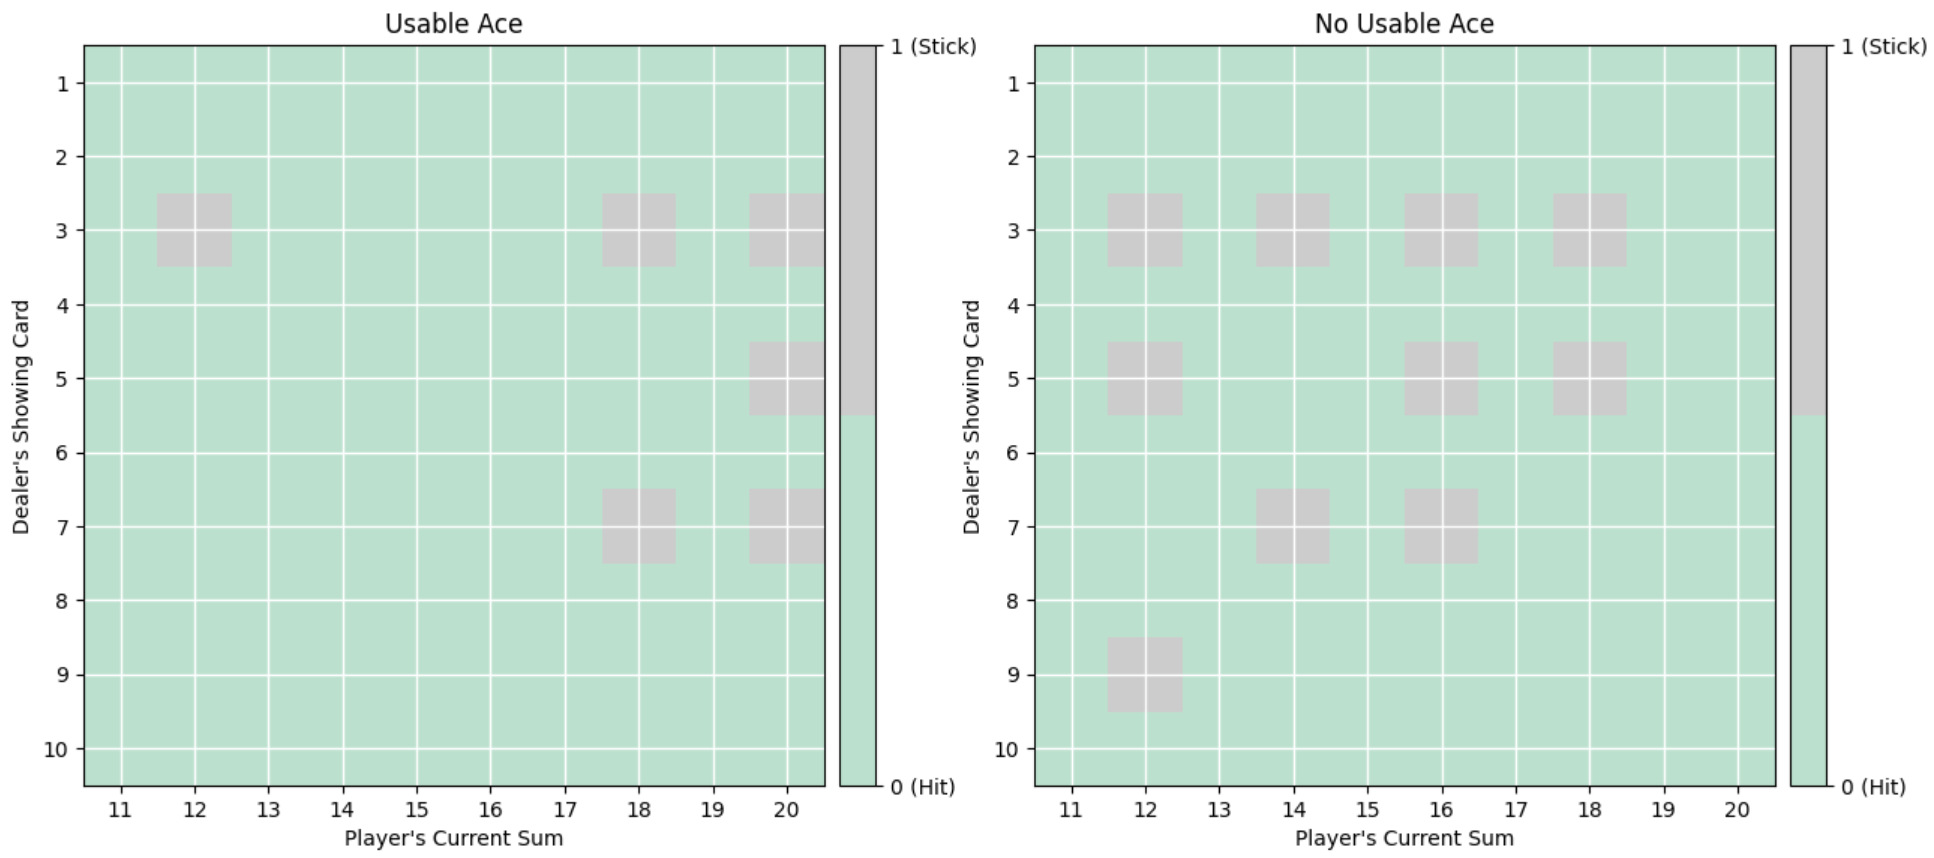
\includegraphics[width=70mm]{figures/Q-Learning/advanced-counting-10-million/policy-some-cards-played-1010101010.png}
	\caption{Q-Learning with advanced counting method. Every other card has been played, starting from Ace. From own calculations.}
	\label{fig:q-learning-advanced-every-other}
\end{figure}

And Figure \ref{fig:q-learning-advanced-every-other} shows the policy for an even more uncommon state which results in a very noise policy. 
Note that the value-function for all states are initialized with 0 and zero is displayed as "Hit" in this plot which makes the policy look less noisy in the plot than it actually is. 



\subsubsection{Deep Q-Learning}
A general note on Deep Q-Learning is that one training iteration takes more time than for the other discussed RL-methods since a neural network has to be trained. 
Secondly, to train a deep neural network a large amount of training iterations are needed. 
Combining these two facts indicates that training Deep Q-Learning takes more time.
The training of the Deep Q-Networks were stopped after 180.000 training episodes due to the extensive training time. 
For that reason, the traditional RL-methods were trained on approximately 1.000 times the magnitude of episodes compared to the Deep Q-Learning method.

\begin{figure}
	\centering
	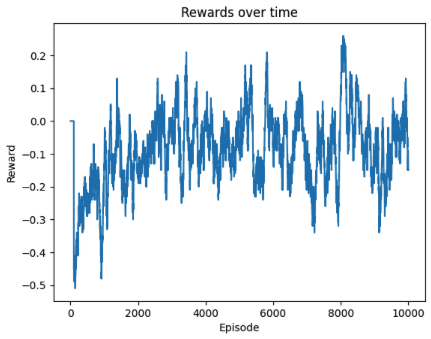
\includegraphics[width=70mm]{figures/DQN/rewards_over_time_10000.png}
	\caption{Deep Q-Learning with advanced counting method. Rewards over the first 10.000 episodes. From own calculations.}
	\label{fig:dqn-rewards-over-time}
\end{figure}

Figure \ref{fig:dqn-rewards-over-time} indicates the DQN's learning within the first 10.000 episodes. 
The learning curve within the first 1.000 is remarkable because of the complex state-space and the complex neural network architecture. 
Although it is important to note that the average reward stays at around -0.1 after.

\begin{figure}
	\centering
	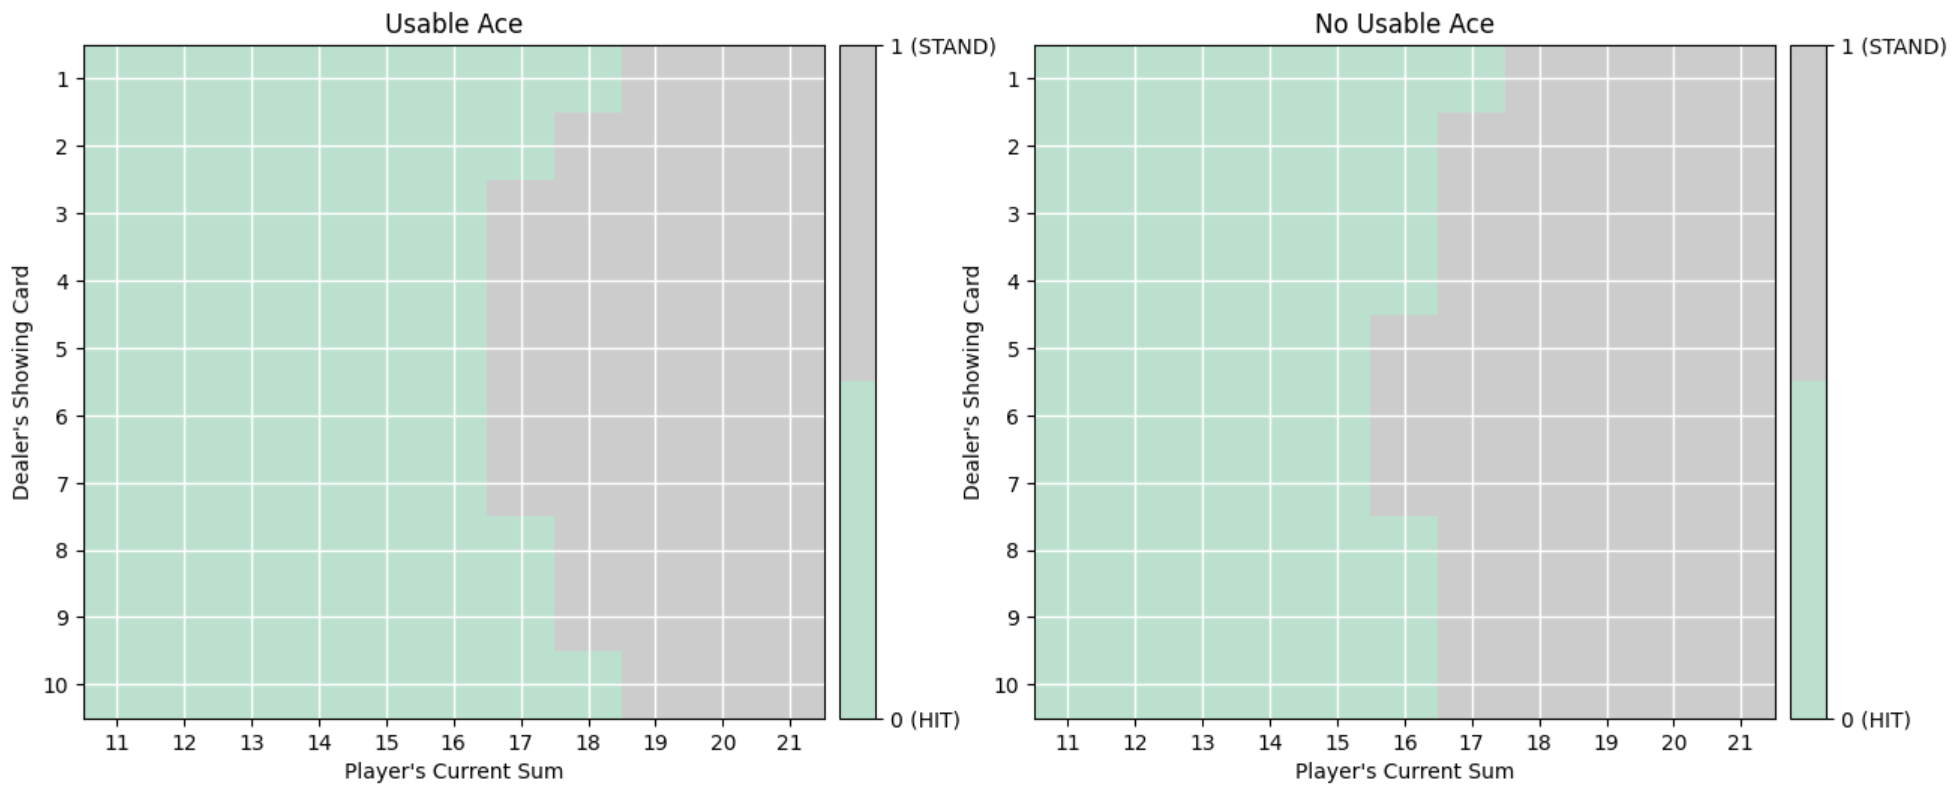
\includegraphics[width=70mm]{figures/DQN/advanced/policy-1010101010.png}
	\caption{Deep Q-Learning with advanced counting method. Every other card has been played, starting from Ace. From own calculations.}
	\label{fig:dqn-advanced-every-other}
\end{figure}

Figure \ref{fig:dqn-advanced-every-other} shows that the Deep Q-learning is able to approximate the policy well even for a very uncommon state. 
Note that the same state was shown in Figure \ref{fig:q-learning-advanced-every-other} for Q-Learning. 
The Deep Q-Learning estimates the policy substantially better for this uncommon state compared to the RL-methods. 

Notably the optimal policy for this uncommon state is unclear since it was not covered in \cite{b1} or \cite{b4}.
In this state an ace has been played while a card with value 10 has not been played. 
Since it is unclear what the exact impact of these two card values is, a prediction for a perfect policy can not be made without further investigation. 
Although the policy seems reasonable since it comes close to the basic strategy \cite{b1} which should logically be a similar state.

\begin{figure}
	\centering
	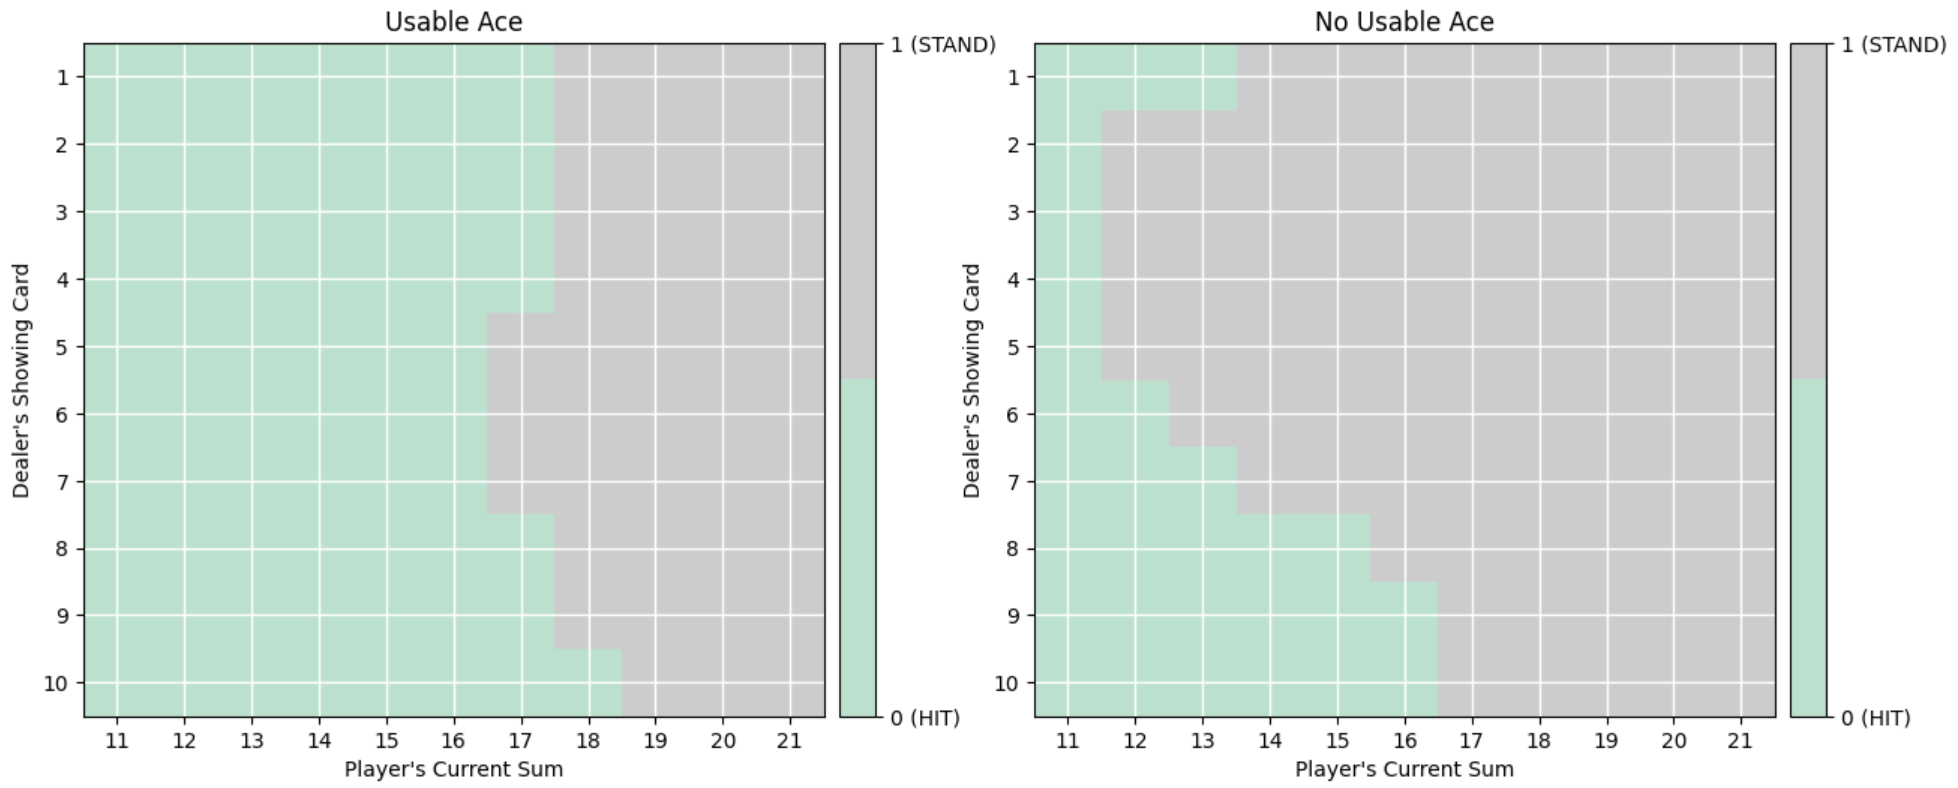
\includegraphics[width=70mm]{figures/DQN/advanced/policy-low-cards-played.png}
	\caption{Deep Q-Learning with advanced counting method. Only low cards (2,3,4,5,6) have been played. From own calculations.}
	\label{fig:dqn-advanced-only-low}
\end{figure}

Figure \ref{fig:dqn-advanced-only-low} shows the policy for the state where only low cards have been played. 
This comes close to a high counting score for the Complete Point Count System in Figure \ref{fig:dqn-card-counting-7}.
Although it is important to note that those two states are not equivalent since the advanced counting method does not keep track of how many cards of a single value have been played.

% TODO: Plots: Vllt. T-SNE plot?


\section{Conclusion}
% TODO: Kurze Zusammenfassung hier?
Summarizing the results, all of RL-methods and the Deep Q-Learning method were able to model the baseline basic strategy from \textit{Beat the dealer} \cite{b1}.

As the state-space was increased to 1.024.000 states, all of the traditional RL-methods (Monte Carlo Control, SARSA and Q-Learning) indicated a struggle to estimate the optimal policy.
Deep Q-Learning on the other hand seemed to handle this high state-space remarably well by estimating the optimal policy well even for very uncommon states.

Further study the following four areas would be interesting:

First, one important note that was already mentioned is that the traditional RL-methods were trained on approximately 1.000 times the magnitude of episodes compared to the Deep Q-Learning.
The training for the Deep Q-Learning was stopped at 180.000 episodes, which took 3 hours and 7 minutes, due to the deadline of this submission.
Interestignly between 120.000 and 180.000 training episodes, the estimated policy improved noticably and it would therefore be interesting to train the DQN further. 

Secondly, in the methods section it was already mentioned that the desired advanced counting method could not be examined due to hardware limitations. 
Although the result with the limited counting method was still insightful, the test should be examined again with better hardware.
With the advanced counting method of keeping track of every played card-value, it would be interesting to test whether the expected reward would exceed the Complete Point Count System \cite{b1}.

Thirdly, the performance of the DQN could be tested when removing its two implementation details: Experience Replay Buffer and Target Neural Network \cite{b2}.
The \textit{Playing Atari with Deep Reinforcement Learning} paper \cite{b2} suggest less robust training in that case but there are no scientific benchmarks, to my knowledge.

Lastly, testing the trained DQN without any further training on other similar card games would be very interesting.
This idea is motivated by the \textit{Playing Atari with Deep Reinforcement Learning} paper where the trained model was able to achieve super-human level of play in different Atari games without any further training \cite{b2}. 


\begin{thebibliography}{00}
\bibitem{b1} Thorp, E. O. (1966). Beat the dealer: A winning strategy for the game of twenty-one (Vol. 310). Vintage.
\bibitem{b2} Mnih, V., Kavukcuoglu, K., Silver, D., Graves, A., Antonoglou, I., Wierstra, D., \& Riedmiller, M. (2013). Playing atari with deep reinforcement learning. arXiv preprint arXiv:1312.5602.
\bibitem{b3} Mnih, V., Kavukcuoglu, K., Silver, D., Rusu, A. A., Veness, J., Bellemare, M. G., ... \& Hassabis, D. (2015). Human-level control through deep reinforcement learning. nature, 518(7540), 529-533.
\bibitem{b4} Sutton, R. S., \& Barto, A. G. (2018). Reinforcement learning: An introduction. MIT press.
\bibitem{b5} Watkins, C. J., \& Dayan, P. (1992). Q-learning. Machine learning, 8, 279-292.
\bibitem{b6} Roderick, M., MacGlashan, J., \& Tellex, S. (2017). Implementing the deep q-network. arXiv preprint arXiv:1711.07478.
\end{thebibliography}
\end{document}
